\section{Descripción estructural de un multiplexor \label{sec:s1}}

\begin{center}
	\begin{minipage}{12cm}
		\begin{tcolorbox}[title=Actividad 1]
			Capturar el código para describir en forma estructural el multiplexor en el lenguaje de su elección. Instanciar el módulo o componente que se encuentre en el mismo archivo. Simular el multiplexor.
		\end{tcolorbox}	
	\end{minipage}
\end{center}

La visualización RTL del multiplexor usando descripción estructural en Verilog se muestra en la \autoref{fig::mux_str_des_rtl}. Como se observa, la implementación se hace con la instanciación de un multiplexor, denominado ``MyMux'', visualizado en el interior del módulo (Ver \autoref{fig::mux_str_des_rtl2}). Las simulaciones se visualizan en la \autoref{fig:for_loop1_vhdl_wavebi}, en donde se muestra que el multiplexor descrito opera de manera correcta.

En los Anexos se localiza la descripción en Verilog de este multiplexor. En el código se tienen dos módulos, siendo el primero el de la jerarquía más alta y en donde se realiza la declaración de las entradas y la salida, para luego instanciar al módulo llamado ``MyMux'' con la etiqueta ``u0''. Cabe señalar que los argumentos de la instancia se deben colocar en el orden correcto. El segundo módulo unicamente es la descripción de un multiplexor sencillo, utilizando el operador condicional ``?''.

\begin{figure}[ht]
	\centering
	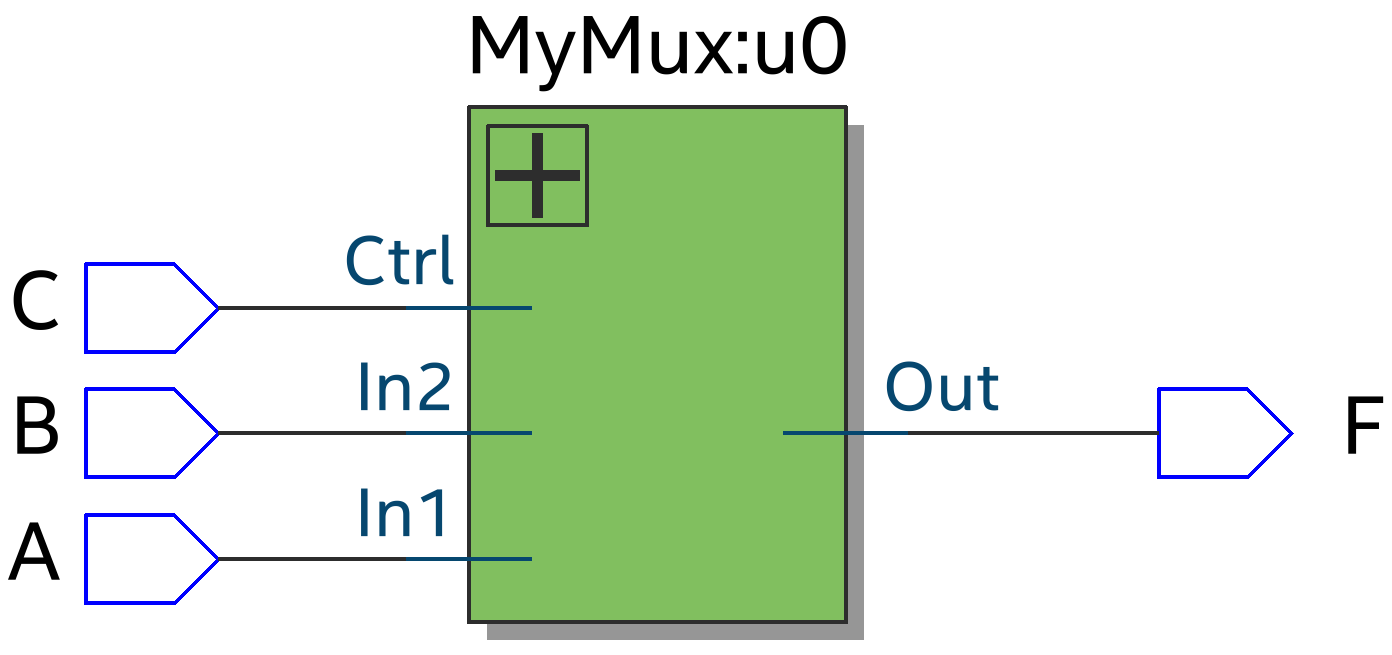
\includegraphics[scale=0.45]{Mux_Structural_Description_RTL.png}
	\caption{Diagrama RTL del multiplexor descrito en forma estructural en Verilog. \label{fig:mux_str_des_rtl}}
\end{figure}

\begin{figure}[ht]
	\centering
	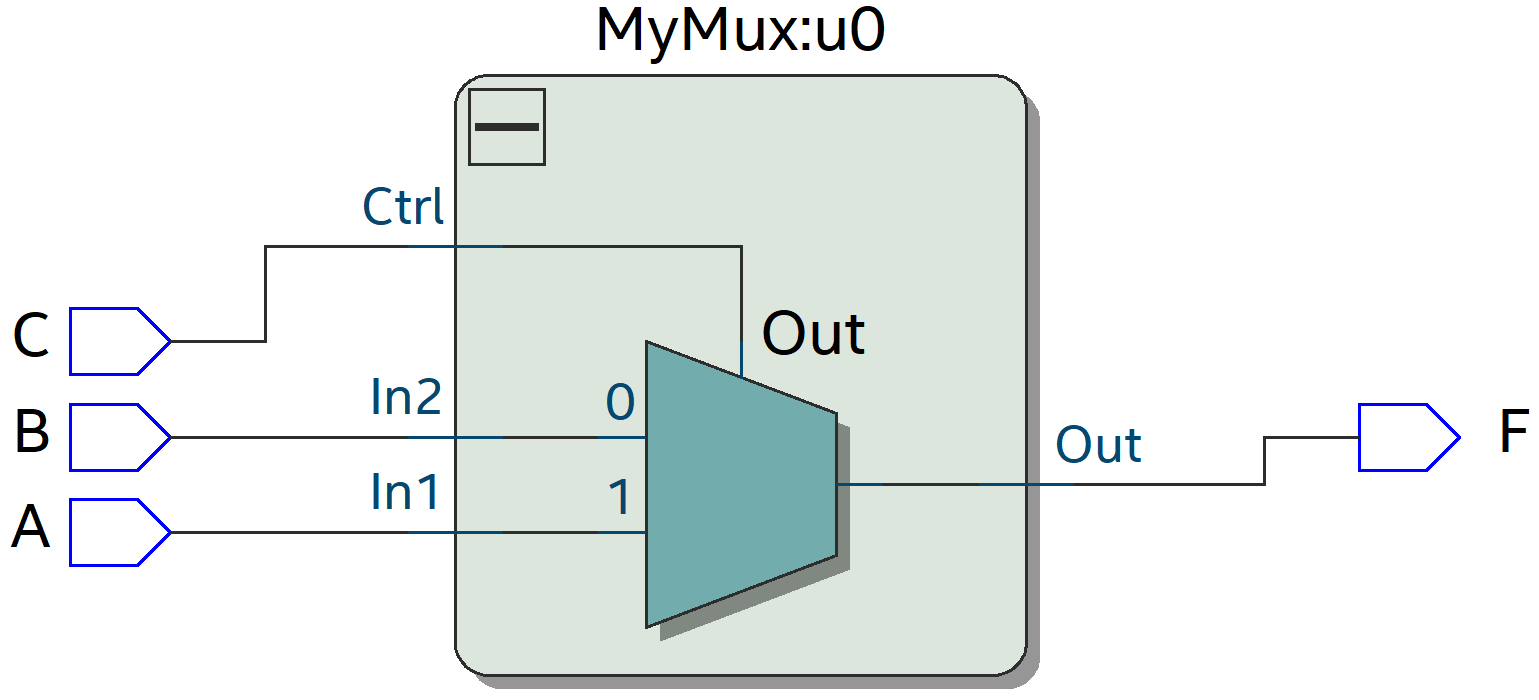
\includegraphics[scale=0.4]{Mux_Structural_Description_RTL2.png}
	\caption{Simulación del multiplexor descrito en forma estructural en Verilog (visualización de la instancia interna). \label{fig:mux_str_des_rtl2}}
\end{figure}

\begin{figure}[ht]
	\centering
	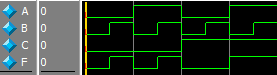
\includegraphics[scale=2]{Mux_Structural_Description_Wave.png}
	\caption{Simulación del multiplexor descrito en forma estructural en Verilog con el visor de formas de onda de ModelSim. \label{fig:mux_str_des_wave}}
\end{figure}